\section*{Kinematics}
\subsection*{Forward Kinematics}
    
\begin{figure}[htbp]
  \centering
  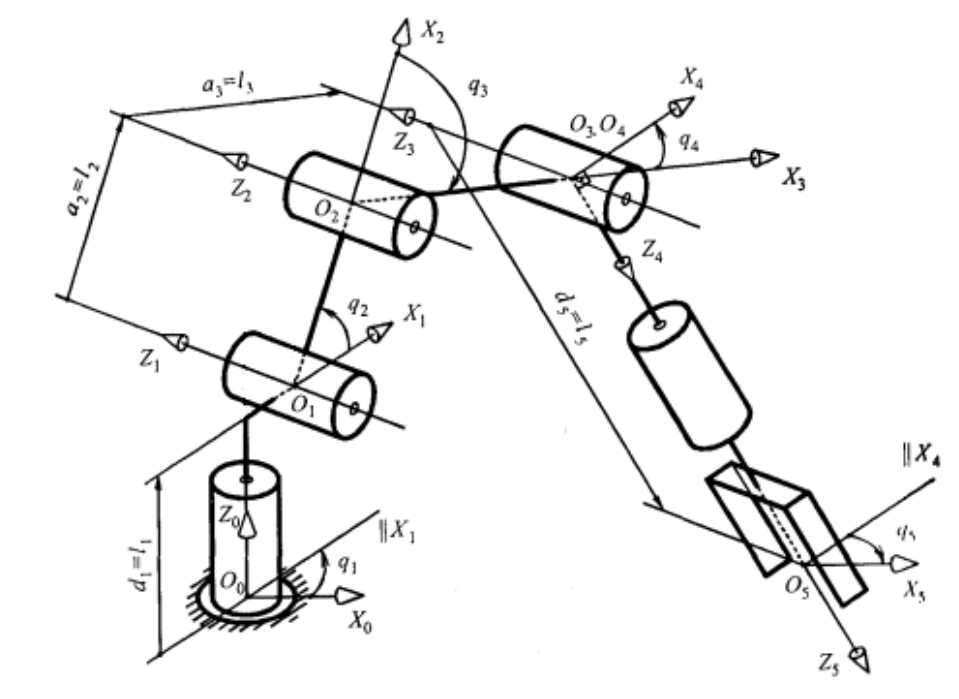
\includegraphics[width=.9\textwidth]{img/DHconv.png}
  \caption{Kinematic scheme of the manipulator. Source \cite{Kinematics}}
  \label{fig:dhf}
\end{figure}

The forward kinematics states the relationship between the end effector and the individual joints. One easy way to get the forward kinematics is to use the Denavit-Hartenberg(DH) convention. \cite{spong} states that each homogenous transformation $A_i$ is represented as a product of four basic transformations: 


$$
A_i = 
    \begin{bmatrix}
        c_{\theta_i} & -s_{\theta_i}c_{\alpha_i} & s_{\theta_i}s_{\alpha_i} & a_ic_{\theta_i}\\
        s_{\theta_i} & c_{\theta_i}c_{\alpha_i} & -c_{\theta_i}s_{\alpha_i} & a_is_{\theta_i}\\
        0 & s_{\alpha_i} & c_{\alpha_i} &d_i\\
        0 & 0 & 0 & 1
    \end{bmatrix}
$$
where $c_{\theta_i} = \cos{(\theta_i)}$ and $s_{\theta_i} = \sin{(\theta_i)}$, and the same for $\alpha$. 
By looking at \figref{fig:dhf} the following DH parametres are found:
\begin{center}
    \begin{tabular}{|c|c|c|c|c|}
         \hline
         Link & $a_i$ & $\alpha_i$ & $d_i$ & $\theta_i$ \\ \hline
         1 & 0 & $-\frac{\pi}{2}$ & $d_1$ & $q_1$ \\
         2 & $a_2$ & 0 & 0 & $q_2$ \\ 
         3 & $a_3$ & 0 & 0 & $q_3$\\
         4 & 0 & $\frac{\pi}{2}$ & 0 & $q_4$\\
         5 & 0 & 0 & $d_5$ & $q_5$\\
         \hline
    \end{tabular}
\end{center}

% d_1 = 0.0506
% a_2 = 0.0506 + 0.0206 + 0.0635 = 0.1347
% a_3 = 0.0506 + 0.0206 = 0.0712
% d_5 = 0.0506 + 0.0206 + 0.0253 + 0.08 = 0.1765

where $d_1 = 0.0506$, $a_2 = 0.1347$, $a_3 = 0.0712$ and $d_5 = 0.1765$ for the model. The real values need to be measured properly since the data sheet of the robot is insufficient. 
Now it is possible to calculate $A_i$ for each joint. Using Matlab:

\begin{align*}
A_1 &= \begin{bmatrix} 
            c_1 & 0 & -s_1 & 0\\
            s_1 & 0 & c_1 & 0\\
            0 & -1 & 0 & d_1\\
            0 & 0 & 0 & 1
        \end{bmatrix},
A_2 = \begin{bmatrix} 
            c_2 & -s_2 & 0 & a_2c_2\\
            s_2 & c_2 & 0 & a_2s_2\\
            0 & 0 & 1 & 0\\
            0 & 0 & 0 & 1
        \end{bmatrix},
A_3 = \begin{bmatrix} 
            c_3 & -s_3 & 0 & a_3c_3\\
            s_3 & c_3 & 0 & a_3s_3\\
            0 & 0 & 1 & 0\\
            0 & 0 & 0 & 1
        \end{bmatrix}\\
A_4 &= \begin{bmatrix} 
            c_4 & 0 & s_4 & 0\\
            s_4 & 0 & -s_4 & 0\\
            0 & 1 & 0 & 0\\
            0 & 0 & 0 & 1
        \end{bmatrix},
A_5 = \begin{bmatrix} 
            c_5 & -s_5 & 0 & 0\\
            s_5 & c_5 & 0 & 0\\
            0 & 0 & 1 & d_5 \\
            0 & 0 & 0 & 1
        \end{bmatrix}
\end{align*}

 and then calculate $T_i^0$ using Matlab:
\begin{subequations}
\begin{align}
    T_1^0 &= A_1 =
    \begin{bmatrix}\label{eq:T1}
        c_1 & 0 & -s_1 & 0\\
        s_1 & 0 & c_1 & 0\\
        0 & -1 & 0 & d_1\\
        0 & 0 & 0 & 1
    \end{bmatrix}\\
    T_2^0 &= A_1A_2 =
    \begin{bmatrix}\label{eq:T2}
        c_1c_2 & -c_1s_2 & -s_1 & a_2c_1c_2\\
        s_1c_2 & -s_1s_2 & c_1 & a_2s_1c_2\\
        -s_2 & -c_2 & 0 & d_1 - a_2s_2\\
        0 & 0 & 0 & 1
    \end{bmatrix}\\
    T_3^0 &= A_1A_2A_3=
    \begin{bmatrix}\label{eq:T3}
        c_{23}c_1 & -c_1s_{23} & -s_1 & c_1(a_3c_{23} + a_2c_2)\\
        c_{23}s_1 & -s_1s_{23} & c_1 & s_1(a_3c_{23} + a_2c_2)\\
        -s_{23} & -c_{23} & 0 & d_1 - a_3s_{23}-a_2s_2\\
        0 & 0 & 0 & 1
    \end{bmatrix}\\
    T_4^0 &= A_1A_2A_3A_4=
    \begin{bmatrix}\label{eq:T4}
        c_1c_{234} & -s_1 & c_1s_{234} & c_1(a_3c_{23} + a_2c_2)\\
        s_1c_{234} & c_1 & s_1s_{234} & s_1(a_3c_{23} + a_2c_2)\\
        -s_{234} & 0 & c_{234} & d_1 - a_3s_{23} - a_2s_2\\
        0 & 0 & 0 & 1
    \end{bmatrix}\\
    \begin{split}
        T_5^0 &= A_1A_2A_3A_4A_5\\ &=
        \begin{bmatrix}\label{eq:T5}
            c_1c_{234}c_5 - s_1s5 & -s_1c_5 - c_1c_{234}s_5 & c_1s_{234} & c_1(a_3c_{23} + a_2c_2 + d_5s_{234})\\
            s_1c_{234}c_5 + c_1s_5 & c_1c_5 - s_1c_{234}s_5 & s_1s_{234} & s_1(a_3c_{23} + a_2c_2 + d_5s_{234})\\
            -s_{234}c_5 & s_{234}s_5 & c_{234} & d_1 - a_3s_{23} - a_2s_2 + d_5c_{234}\\
            0 & 0 & 0 & 1
        \end{bmatrix}
    \end{split}
 \end{align}
\end{subequations}
where $s_{ijk} = \sin{(q_i + q_j + q_k)}$ and the same for $c_{ijk}$. The $T_i^0$ matrix can be sectioned into \begin{align*}
 T_i^0 = 
    \begin{bmatrix}
        \bm{R}(\bm{q}) & \bm{p}(\bm{q})\\
        \bm{0}^T & 1
    \end{bmatrix}    
\end{align*}







%-----------------------------------------------------------------------------------------
\begin{comment}
\begin{align*}
    T^0_5 &= A_1A_2A_3A_4A_5\\
    &= 
    \begin{bmatrix}
        c_1c_{234}c_5 + s_1s_5 & -c_1c_{234}s_5+s_1c_5 & -c_1s_{234} & c_1(-d_5s_{234} + a_3c_{23} + a_2c_2)\\
        c_1c_{234}c_5 - s_1s_5 & -s_1c_{234}s_5-c_1c_5 & -s_1s_{234} & s_1(-d_5s_{234} + a_3c_{23} + a_2c_2) \\
        -s_{234}c_5 & s_{234}s_5 & -c_{234} &d_1 - a_2s_2 - a_3s_{23} - d_5c_{234}\\
        0 & 0 & 0 & 1\\
    \end{bmatrix}\\
    &=
    \begin{bmatrix}
        \bm{R}(\bm{q}) & \bm{p}(\bm{q})\\
        \bm{0}^T & 1
    \end{bmatrix}
\end{align*}
\end{comment}
%-----------------------------------------------------------------------------------------









\subsection*{Inverse Kinematics}
\cite{Siciliano} states that one can use the Jacobian of the system to calculate the inverse kinematics:

\begin{align}\label{eq:algo}
\dot{\bm{e}} = \dot{\bm{x}}_d - \bm{J}_A(\bm{q})\dot{\bm{q}}
\end{align}

In \figref{fig:inverseAlgo} the inverse kinematics algorithm is stated. From the figure one can see that 
$$
\dot{\bm{q}} = \bm{J}_A^{-1}(\bm{q})(\dot{\bm{x}}_d + \bm{K}e)
$$
where K is a positive definite diagonal matrix which makes the resulting system \eqref{eq:algo} into the linear system
\begin{align*}
    \dot{\bm{e}} + \bm{K}e = \bm{0}
\end{align*}


\begin{figure}[htbp]
  \centering
  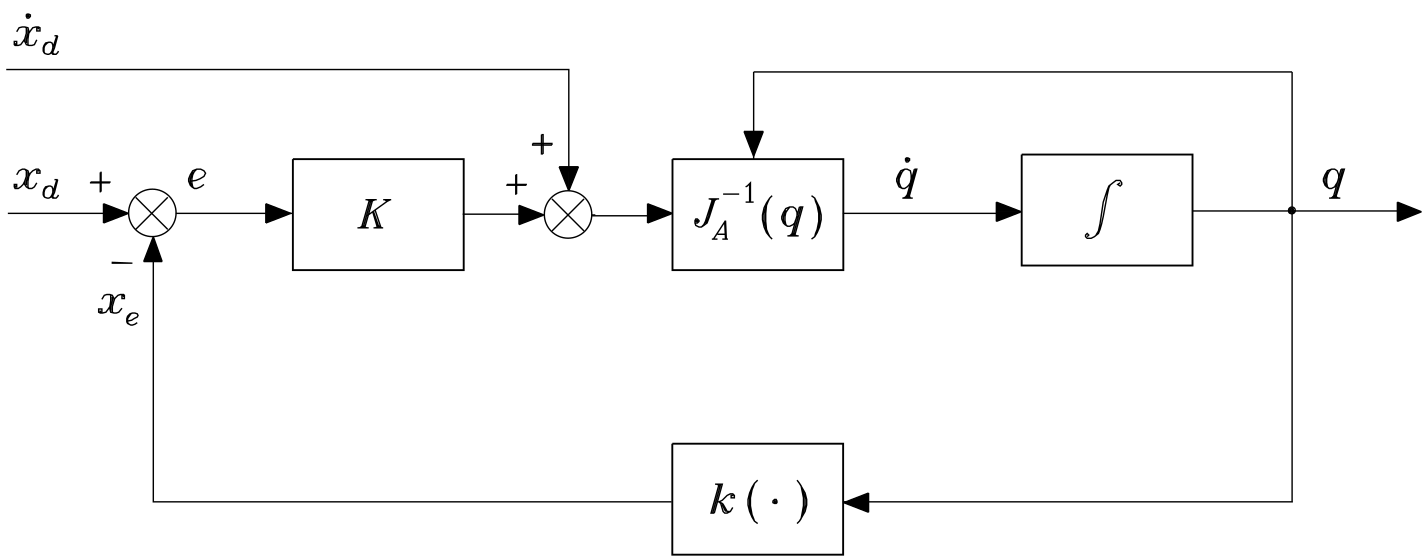
\includegraphics[width=.9\textwidth]{img/inverseKin.png}
  \caption{Inverse kinematics algotihm with Jacobian inverse. Source \cite{Siciliano}.}
  \label{fig:inverseAlgo}
\end{figure}


\subsubsection*{Jacobian}
As we already know the forward/direct kinematics can be written as:
\begin{align*}
    \bm{T}(\bm{q}) = 
    \begin{bmatrix}
        \bm{R}(\bm{q}) & \bm{p}(\bm{q})\\
        \bm{0}^T & 1
    \end{bmatrix}
\end{align*}
we want to express the linear velocity $\dot{\bm{p}}$ and angular velocity $\bm{\omega}$ as a function of the joint velocities $\dot{\bm{q}}$. In \cite{Siciliano} the relations is states as:

\begin{equation}
    \begin{aligned}\label{eq:velo}
        \dot{\bm{p}} &= \bm{J}_P(\bm{q})\dot{\bm{q}}\\
        \bm{\omega} &= \bm{J}_O(\bm{q})\dot{\bm{q}}
    \end{aligned}
\end{equation}

where $\bm{J}_O$ with dimensions (3 $\times$ n) is the relation between the joint velocities $\dot{\bm{q}}$ and the end-effector linear velocity $\dot{\bm{p}}$, and the (3 $\times$ n) matrix $\bm{J}_O$ is the relation between the joint velocities $\dot{\bm{q}}$ and the end-effector angular velocity $\bm{\omega}$. \eqref{eq:velo} can be written as

\begin{align*}
    \bm{v_e} = 
    \begin{bmatrix}
        \dot{\bm{p}} \\ \bm{\omega}
    \end{bmatrix}
    = \bm{J}(\bm{q})\dot{\bm{q}}
\end{align*}
where
\begin{align*}
    \bm{J} = 
    \begin{bmatrix}
        \bm{J}_P \\ \bm{J}_O
    \end{bmatrix}
\end{align*}

which is the matrix that \cite{Siciliano} calls the geometric Jacobian. The elements of 
$$
\bm{J} = 
\begin{bmatrix}
    \bm{j}_{P1} & & \bm{j}_{Pn}\\
    &...&\\
    \bm{j}_{O1} & & \bm{j}_{On}
\end{bmatrix}
$$
can be calculated in the following way:
\begin{align*}
    \begin{bmatrix}
        \bm{j}_{Pi}\\\bm{j}_{Oi}
    \end{bmatrix}
    =
    \begin{cases}
        \begin{bmatrix} \bm{z}_{i-1}\\ \bm{0} \end{bmatrix} & \text{for a prismatic joint}\\
        \begin{bmatrix} \bm{z}_{i-1} \times (\bm{p}_e-\bm{p}_{i-1}) \\ \bm{z}_{i-1} \end{bmatrix} & \text{for a revolute joint}
    \end{cases}
\end{align*}

Since our manipulator only has revolute joints, the geometric Jacobian becomes

\begin{align*}
    \bm{J}(\bm{q}) = 
    \begin{bmatrix}
        \bm{z}_0 \times (\bm{p}_5-\bm{p}_0) & 
        \bm{z}_1 \times (\bm{p}_5-\bm{p}_1) & 
        \bm{z}_2 \times (\bm{p}_5-\bm{p}_2) & 
        \bm{z}_3 \times (\bm{p}_5-\bm{p}_3) & 
        \bm{z}_4 \times (\bm{p}_5-\bm{p}_4) \\
        \bm{z}_0 &
        \bm{z}_1 &
        \bm{z}_2 &
        \bm{z}_3 &
        \bm{z}_4
    \end{bmatrix}
\end{align*}
From when the forward kinematics were calculated each position vector $\bm{p}_i$ can be directly obtained from the equations \eqref{eq:T1} - \eqref{eq:T5}:



\begin{align*}
    \bm{p_0} = \begin{bmatrix} 0 \\ 0 \\ 0 \end{bmatrix}    \quad
    \bm{p_1} = \begin{bmatrix} 0 \\ 0 \\ d_1\end{bmatrix}    \quad
    \bm{p_2} = \begin{bmatrix} a_2c_1c_2\\ a_2s_1c_2\\ d_1 - a_2s_2\end{bmatrix}   \quad 
    \bm{p_3} = \begin{bmatrix} c_1(a_3c_{23} + a_2c_2) \\ s_1(a_3c_{23} + a_2c_2) \\ d_1 - a_3s_{23}-a_2s_2 \end{bmatrix}  \\  
    \bm{p_4} = \begin{bmatrix} c_1(a_3c_{23} + a_2c_2) \\ s_1(a_3c_{23} + a_2c_2) \\ d_1 - a_3s_{23}-a_2s_2\end{bmatrix}  \quad  
    \bm{p_5} = \begin{bmatrix} c_1(a_3c_{23} + a_2c_2 + d_5s_{234}) \\ s_1(a_3c_{23} + a_2c_2 + d_5s_{234}) \\ d_1 - a_3s_{23} - a_2s_2 + d_5c_{234} \end{bmatrix}    
\end{align*}

The next step is to find $z_{i-1}$. \cite{Siciliano} states that $\bm{z}_{i-1}$ is given by the third column of the rotation matrix $\bm{R}_{i-1}^0$. $\bm{R}_{i-1}^0$ is already given in $T_i^0$, By looking at \eqref{eq:T1} - \eqref{eq:T5} the following values of $z_{i-1}$ is given:
\begin{align*}
    z_0 &= \begin{bmatrix}0\\0\\1\end{bmatrix},
    z_1 = \begin{bmatrix}-s_1\\c_1\\0\end{bmatrix},
    z_2 = \begin{bmatrix}-s_1\\c_1\\0\end{bmatrix},
    z_3 = \begin{bmatrix}-s_1\\c_1\\0\end{bmatrix},
    z_4 = \begin{bmatrix}c_1s_{234}\\s_1s_{234}\\c_{234}\end{bmatrix}
\end{align*}

now we got everything needed to compute the geometric Jacobian. The symbolic calculation is done in Matlab:


\begin{align*}
    \bm{J}(\bm{q}) &= \\
    &\begin{bmatrix}
        -s_1(a_3c_{23} + a_2c_{2} + d_5s_{234}) & 
        -c_1(a_3s_{23} + a_2s_{2} - d_5c_{234}) & 
        -c_1(a_3s_{23} - d_5c_{234})            & 
        c_1d_5c_{234}                           & 
        0\\
        c_1(a_3c_{23} + a_2c_{2} + d_5s_{234})  & 
        -s_1(a_3s_{23} + a_2s_{2} - d_5c_{234}) & 
        -s_1(a_3s_{23} - d_5c_{234})            & 
        s_1d_5c_{234}                           & 
        0\\
        0                                       &
        -a_3c_{23}- a_2c_2 - d_5s_{234}         &
        -a_3c_{23} - d_5s_{234}                 &
        -d_5s_{234}                             &
        0\\
        0                                       &
        -s_1                                    &
        -s_1                                    &
        -s_1                                    &
        c_1s_{234}\\
        0                                       &
        c_1&
        c_1&
        c_1&
        s_1s_{234}\\
        1& 0 & 0 & 0 & c_{234}
    \end{bmatrix}
\end{align*}
which has the full rank of $5$. 
\subsubsection*{Analytical Jacobian}
To use the algorithm in \figref{fig:inverseAlgo} the analytical Jacobian is needed. In \cite{Siciliano} the following relationship is given
\begin{align*}
    \bm{J}_A =
    \begin{bmatrix}
        \bm{I} & \bm{0}\\ 0 & \bm{T}^{-1}(\bm{\phi_e})
    \end{bmatrix}
    \bm{J}(\bm{q})
\end{align*}

where $\bm{\phi_e} = [\phi,\theta,\psi]^T$ is the orientation of the end-effector frame relative to the base frame given by the Euler angles ZYZ. From \eqref{eq:T5} the rotation matrix from the base frame to end-effector is
\begin{align*}
    \bm{R}_5^0 &= 
    \begin{bmatrix}
        r_{11} & r_{12} & r_{13}\\
        r_{21} & r_{22} & r_{23}\\
        r_{31} & r_{32} & r_{33}
    \end{bmatrix}
    =
    \begin{bmatrix}
        c_1c_{234}c_5 - s_1s_5 & -s_1c_5 - c_1c_{234}s_5 & c_1s_{234}\\
        s_1c_{234}c_5 + c_1s_5 & c_1c_5 - s_1c_{234}s_5 & s_1s_{234}\\
        -s_{234}c_5 & s_{234}s_5 & c_{234} 
    \end{bmatrix}
\end{align*}

The ZYZ Euler angles are then


\begin{align*}
    \phi &= atan2(r_{21},r_{11}) = atan2(s_1c_{234}c_5 + c_1s_5,c_1c_{234}c_5 - s_1s_5)\\
    \theta &= atan2\left(-r_{31},-\sqrt{r_{32}^2+r_{33}^2}\right) = atan2\left(s_{234}c_5,-\sqrt{s_{234}s_5^2+c_{234}^2}\right)\\
    \psi &= atan2(r_{32},r_{33}) = atan2(s_{234}s_5,c_{234})
\end{align*}

The angular velocity $\bm{\omega}_e$ and $\bm{T}(\bm{\alpha})$ is given as

\begin{align*}
    \bm{\omega} = 
    \begin{bmatrix}
        0 & -s_\phi & c_\phi s_\theta\\
        0 & c_\phi & s_\phi s_\theta\\
        1 & 0 & c_\theta
    \end{bmatrix}
    \begin{bmatrix}
        \dot{\phi}\\\dot{\theta}\\\dot{\psi}
    \end{bmatrix}
    =
    \bm{T}(\bm{\phi}_e)\dot{\bm{\phi}}_e
\end{align*}
The determinant of $\bm{T}$ is $-s_\theta$ which means that one cannot invert for $\theta = 0,\pi$. This singularity is also the singularity of the geometric Jacobian. 














































%\begin{comment}
If the desired position is $p$ and the desired orientation is $R$. Then in \cite{Kinematics}, the inverse kinematics are given as: 

\begin{align*}
    q_1 &= \tan^{-1}{\left(\frac{p_y}{p_x}\right)}\\
    q_2 &= atan2\left( a(a_2+a_3c_3) - ba_3s_3, aa_3s_3 + b(a_2+a_3c_3) \right)\\%atan2
    q_3 &= \cos^{-1}{\left(\frac{a^2+b^2-a^2_2-a^2_3}{2a_2a_3}\right)}\\
    q_4 &= q_{234} - q_2 - q_3\\
    q_5 &= c_{234}q_1-2atan(R_{21},R_{11})
\end{align*}

where $a = d_1 - d_5c_{234}-p_z$, $b = p_xc_1 + p_ys_1+d_5s_{234}$ and $-\frac{\pi}{2}<q_1 < \frac{\pi}{2}$. $q_{234} = atan2\left(\frac{p_x}{c_1p_x+s_1p_y})\right)$

%\cite{Siciliano}
%\end{comment}
